\documentclass{beamer}
\usepackage{default}
\usepackage{pgfpages}
\usepackage{tikz}
\usepackage{mathtools}
\renewcommand{\thefootnote}{}
\usepackage{colortbl}
\usepackage{hyperref}
\usepackage{multimedia}
\title{Git Review}
\begin{document}


\begin{frame}
\begin{center}
Introduction to Version Control with \texttt{Git}
\end{center}
\end{frame}

\begin{frame}
\frametitle{Why do I need version control?}
\end{frame}


\begin{frame}
\frametitle{Why do I need version control?}
\begin{center}
\scalebox{0.4}{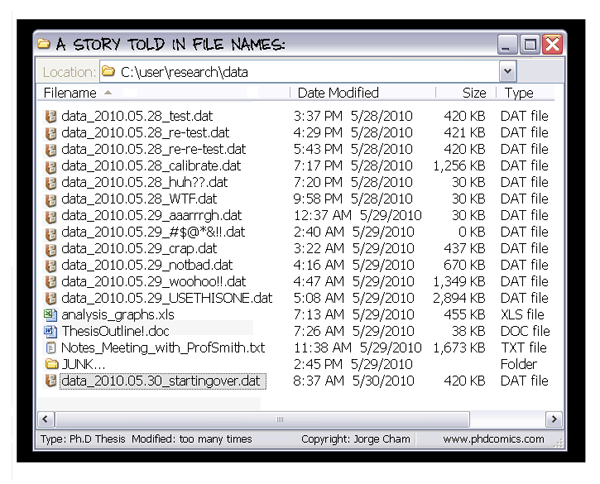
\includegraphics{imgs/version_control.png}}
\end{center}
\footnote{\footnotesize{https://www.phdcomics.com}}
\end{frame}

\begin{frame}
\frametitle{Why do I need version control?}

\end{frame}

\begin{frame}
\frametitle{\texttt{Git}}

\end{frame}

\begin{frame}
\frametitle{\texttt{Git} Workflow}

\end{frame}

\end{document}


